\documentclass{JECnew}
\usepackage[T1]{fontenc}
\usepackage{textcomp}
\usepackage[sc]{mathpazo}
\usepackage[utf8]{inputenc}
\usepackage{amsmath,amsxtra,amssymb,amsthm,latexsym,amscd,amsfonts,mathtools}
\usepackage{multicol}
\usepackage{booktabs,multirow}
\usepackage{setspace}
\usepackage{graphicx}
\usepackage{xcolor}
\usepackage[square, comma, numbers, sort&compress]{natbib}
\usepackage{balance}
\usepackage{tabulary}
\usepackage{subfigure}
\usepackage{soul,color}
\usepackage{textgreek}
\usepackage[noabbrev,capitalize,nameinlink]{cleveref}
\usepackage{gensymb}
\usepackage{siunitx}
\usepackage{float}
\usepackage{lettrine}
\usepackage{url}

\newcolumntype{P}[1]{>{\centering\arraybackslash}p{#1}}
\newcolumntype{R}[1]{>{\raggedleft\arraybackslash}p{#1}}

\raggedbottom
\addtolength{\textheight}{20pt}
\setlength{\footskip}{0.25in}
\setlength{\intextsep}{4pt}
\setlength{\columnsep}{0.25in}

\setlength{\parindent}{0pt}
\renewcommand{\LettrineFontHook}{\bfseries}
\setlength{\DefaultFindent}{-0.1em}

%%%%%%%%%%%%%%%%%%%%%%%%%%%%%%%%%%%%%%%%%%%%%%%%%%%%%%%%%%%%%%%%%%%%%%%%
\definecolor{blue}{rgb}{0,0,0}
\begin{document}

\IEEEspecialpapernotice{Regular Article}
\title{Intelligent AutoEncoder-Based Modulation: Optimizing Transmission Performance over Non-Ideal Wireless Channels}

\author{%
Lai Tien De$^1$, Pham Xuan Nghia$^1$, and Tran Trung Duc$^2$
    \JECaffiliation{$^1$ Faculty of Radio-Electronics Engineering, Le Quy Don Technical University, Hanoi, Vietnam\\
    $^2$ Center for Standards, Metrology and Quality, Vietnam}
    \JECcorrespondence{Pham Xuan Nghia, Faculty of Radio-Electronics Engineering, Le Quy Don Technical University, Hanoi, Vietnam. Email: nghiapx@lqdtu.edu.vn}
    \JECcommunication{received --, revised --, accepted --}
    \JECeditor{Prof. --}
    \JEConlineDate{--}
    \JEConlineDOI{10.21553/rev-jec.xxx}
}

\IEEEcompsoctitleabstractindextext{%
\begin{abstract}
This paper presents an End-to-End wireless transceiver based on deep AutoEncoder (AE) networks that jointly optimizes the transmitter and receiver as a single differentiable system, replacing the conventional cascade of independently designed signal processing blocks. The physical channel model incorporates three concurrent impairments: power amplifier (PA) nonlinearity (Rapp model), carrier frequency offset (CFO), and Rayleigh fading. Three AE architectures of increasing complexity are proposed and validated. Specifically, a single-symbol AE learns a PA-resilient constellation, achieving a $3$--$4$~dB SNR gain over 16-QAM with ZF equalization. Furthermore, a multi-symbol AE performs blind CFO compensation without PLLs or pilots, yielding a $5$--$8$~dB gain. Finally, a Neural FEC architecture unifies modulation and channel coding, providing reliable error correction on composite degraded channels. Monte Carlo simulations confirm that the proposed architectures outperform conventional block-wise approaches under complex nonlinear channel conditions.\end{abstract}
\begin{keywords}
AutoEncoder, Intelligent physical layer, Deep Learning, Digital modulation, Forward Error Correction, Power Amplifier nonlinearity, Carrier Frequency Offset.
\vspace{-8pt}
\end{keywords}
}

\maketitle
\setcounter{page}{1}

\makeatletter
\def\ps@firstpage{%
  \def\@oddfoot{\hfill\scriptsize 1859-378X--2025-xxxx~\copyright~2025 REV\hfill}%
  \def\@evenfoot{\hfill\scriptsize 1859-378X--2025-xxxx~\copyright~2025 REV\hfill}%
}
\makeatother
\thispagestyle{firstpage}

\renewcommand{\leftmark}{{\small REV Journal on Electronics and Communications: \textit{Article scheduled for publication}}}
\renewcommand{\rightmark}{\small \textbf{Lai \MakeLowercase{\textit{et al.}}:} Intelligent AutoEncoder-Based Modulation}

%-----------------------------------------------------------------------

\section{Introduction}

\lettrine[lines=2, loversize=0.15, findent=0.1em]{I}{n} digital communication systems, modulation is the process of converting discrete data streams into continuous waveform signals suitable for the physical channel characteristics, accomplished by mapping them onto the complex IQ plane. Since this mapping involves a nonlinear transformation from a discrete bit space to a continuous signal space, it can be closely approximated by artificial neural networks~\cite{hornik1991}. Conventional modulation schemes are typically designed under the assumption of ideal or AWGN-only channels. In practical deployments, the transmitted signal simultaneously encounters nonlinear distortion from the power amplifier (PA), carrier frequency offset (CFO), and multipath fading. Higher-order modulation formats that encode information in the signal phase, such as M-PSK and M-QAM, are particularly vulnerable to these impairments~\cite{proakis2008}. Traditional approaches treat each impairment with independent processing blocks (PLL, ZF/MMSE equalizer, PAPR reduction), yielding sub-optimal end-to-end performance due to the lack of global optimization~\cite{oshea2017}.

O'Shea and Hoydis~\cite{oshea2017} first showed that a complete communication link can be cast as an AutoEncoder (AE): the transmitter acts as the encoder, the channel as a stochastic layer, and the receiver as the decoder, enabling joint optimization of all parameters under a single loss function. Subsequent work has expanded in several directions, including {\color{blue}deep learning-based constellation shaping~\cite{stark2019} and hardware prototype deployment~\cite{cammerer2020}. Recently, Aoudia and Hoydis~\cite{aoudia2022} extended the AE End-to-End concept to pilotless OFDM systems, Hoydis et al.~\cite{hoydis2024} developed a differentiable channel simulation platform, and Wiesmayr et al.~\cite{wiesmayr2025} demonstrated a standard-compliant real-time neural receiver for 5G NR, confirming the practical feasibility of neural End-to-End transceivers in deployed cellular networks.}

{\color{blue}However, the majority of existing studies consider only ideal AWGN channels or treat individual impairments in isolation. The combined effect of severe PA nonlinearity, progressive CFO phase rotation, and multipath Rayleigh fading on AE-based transceivers remains largely unexplored. Furthermore, the ability of a single unified neural network to jointly perform modulation, impairment compensation, and forward error correction (FEC) under these composite conditions has not been systematically investigated.}

{\color{blue}This paper proposes an End-to-End differentiable transceiver architecture and evaluates its performance on complex composite channels. The main contributions are summarized as follows:}
\begin{itemize}
    {\color{blue}\item \textbf{PA-Resilient Constellation Shaping:} A single-symbol AE autonomously learns an optimal constellation layout within the PA linear region, reducing PAPR and achieving a 3--4~dB SNR gain over 16-QAM with ZF equalization under strong PA saturation.}
    {\color{blue}\item \textbf{Multi-Symbol AE Architecture with Time-Distributed Encoder:} A multi-symbol AE extends the single-symbol model using a Time-Distributed Encoder to process a block of $L$ symbols. The Decoder observes the entire received sequence, exploiting inter-symbol correlations (CFO phase drift, slow fading) to improve decoding performance. This architecture serves as the foundation for both blind CFO compensation and Neural FEC.}
    {\color{blue}\item \textbf{Blind CFO Compensation via Sequence Learning:} Building on the multi-symbol architecture, the deep decoder observes cumulative phase rotation across a symbol block, performing robust blind CFO estimation without PLLs or pilot overhead, attaining a 2--3~dB gain over conventional 16-QAM.}
    {\color{blue}\item \textbf{Unified Modulation and Neural FEC:} The multi-symbol AE architecture is further extended to integrate channel coding by mapping input bits into multi-symbol blocks with redundancy, eliminating the traditional boundary between modulation and error correction, with BER below $10^{-4}$ at low SNR over composite non-ideal channels.}
    {\color{blue}\item \textbf{Training Framework and System Compatibility:} Multi-phase curriculum learning with physics-constrained loss functions ($\lambda_P$, $\lambda_D$) enables stable convergence over nonlinear channels. Softmax outputs provide soft LLR extraction, ensuring compatibility with modern iterative decoders (Turbo, LDPC).}
\end{itemize}

{\color{blue}The remainder of this paper is organized as follows: Section~II presents the fundamentals of digital modulation and non-ideal channel models. Section~III details the proposed AutoEncoder architectures. Section~IV describes the curriculum training methodology. Section~V presents Monte Carlo simulation results. Finally, Section~VI concludes the paper.}

\section{Digital Modulation Fundamentals and Non-Ideal Channel Conditions}

\subsection{Principles of Digital Modulation}

Digital modulation is the process of transforming a binary data bit stream into a waveform signal suitable for transmission over a physical channel. At the modulator, each group of $k = \log_2 M$ bits is mapped to a symbol corresponding to a point on the constellation diagram in the complex IQ signal plane. The baseband signal of the $n$-th symbol is expressed as:
\begin{equation}
x[n] = a_I[n] + j \cdot a_Q[n]
\end{equation}
where $a_I[n]$ and $a_Q[n]$ are the in-phase and quadrature components, respectively, determined by the constellation mapping table of the modulation scheme.

In M-PSK, information is encoded in the signal phase with constant amplitude: $x_m = A \cdot e^{j2\pi m/M}$. In M-QAM, information is encoded in both amplitude and phase on a regular IQ grid. Higher modulation order $M$ improves spectral efficiency but reduces the minimum Euclidean distance $d_{\min}$ between constellation points.

At the receiver, the demodulator performs hard decision by identifying the nearest constellation point to the received signal in terms of Euclidean distance:
\begin{equation}
\hat{m} = \arg\min_{m \in \{0,\ldots,M-1\}} \| y - x_m \|^2
\end{equation}
The symbol error probability depends directly on the ratio $d_{\min}^2 / N_0$, where $N_0$ is the noise power spectral density.

\subsection{Non-Ideal Channel Conditions}

In practice, wireless signals are simultaneously affected by multiple impairments. This subsection analyzes the three categories investigated in this study.

\subsubsection{Power Amplifier (PA) Nonlinear Distortion}
The power amplifier at the transmitter, when operated near its saturation region to maximize power efficiency, introduces nonlinear distortion to the signal. The Rapp model characterizes the PA's AM/AM and AM/PM behavior:
\begin{equation}
g(r) = \frac{r}{\left(1 + \left(\frac{r}{A_{sat}}\right)^{2p}\right)^{1/2p}}, \quad \Phi(r) = \frac{{\color{blue}\alpha_{PM}} r^2}{1 + {\color{blue}\beta_{PM}} r^2}
\end{equation}
where $r = |x|$ is the input amplitude, $A_{sat}$ is the saturation amplitude, $p$ controls the transition smoothness{\color{blue}, and $\alpha_{PM}$, $\beta_{PM}$ are AM/PM conversion coefficients}. As shown in \textbf{Figs.~\ref{fig:pa_curve}--\ref{fig:qam_pa}}, output amplitude saturates beyond $A_{sat}$, compressing outer 16-QAM symbols by $\sim$1~dB and reducing $d_{\min}$.

\begin{figure}[H]
    \centering
    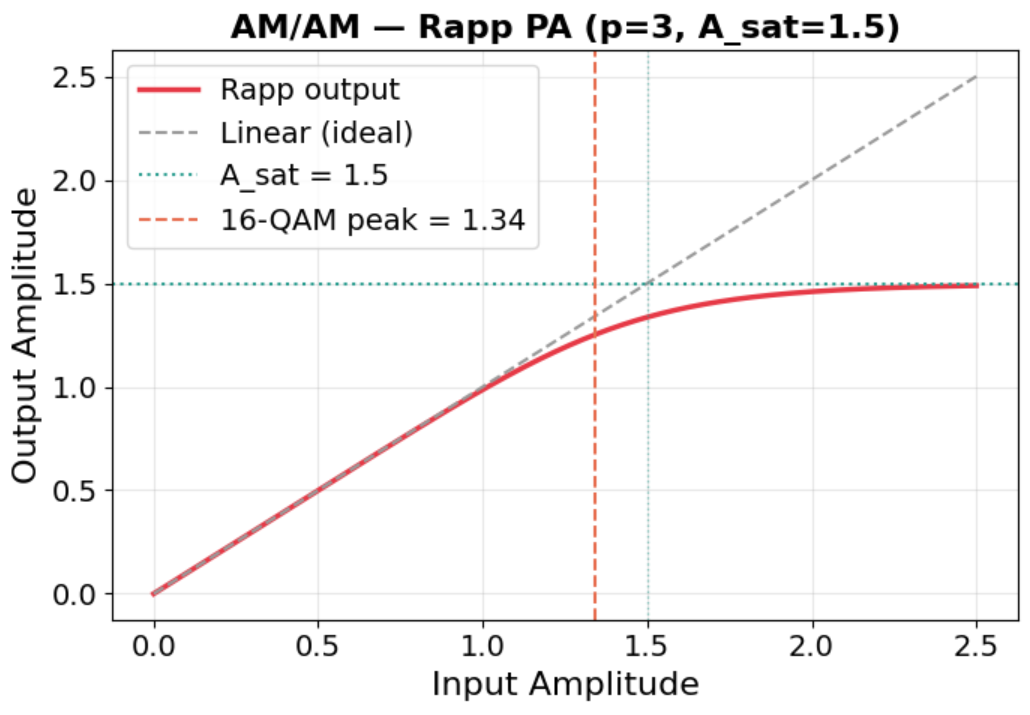
\includegraphics[width=0.98\linewidth]{images/PA characteristic curve 1.png}\\[1ex]
    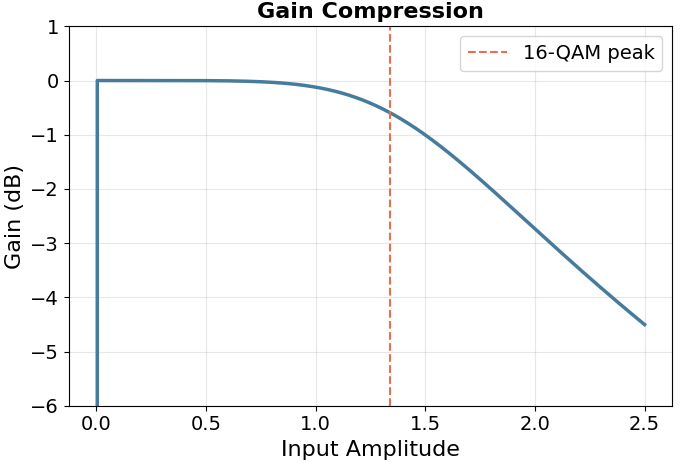
\includegraphics[width=0.98\linewidth]{images/PA characteristic curve 2.png}
    \caption{PA response characteristics modeled under the Rapp format.}
    \label{fig:pa_curve}
\end{figure}

\begin{figure}[H]
    \centering
    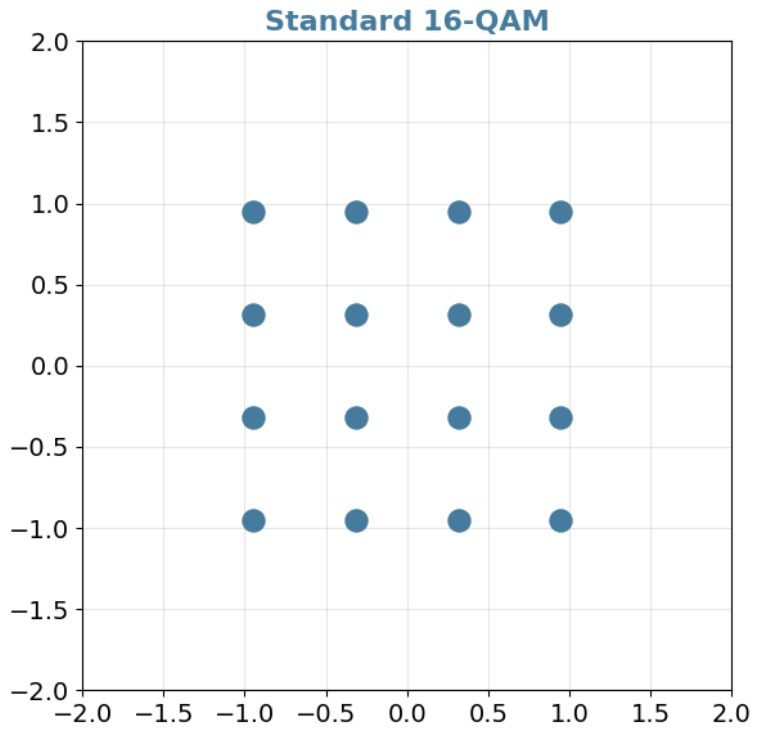
\includegraphics[width=0.48\linewidth]{images/16QAM-constellation.png}\hfill
    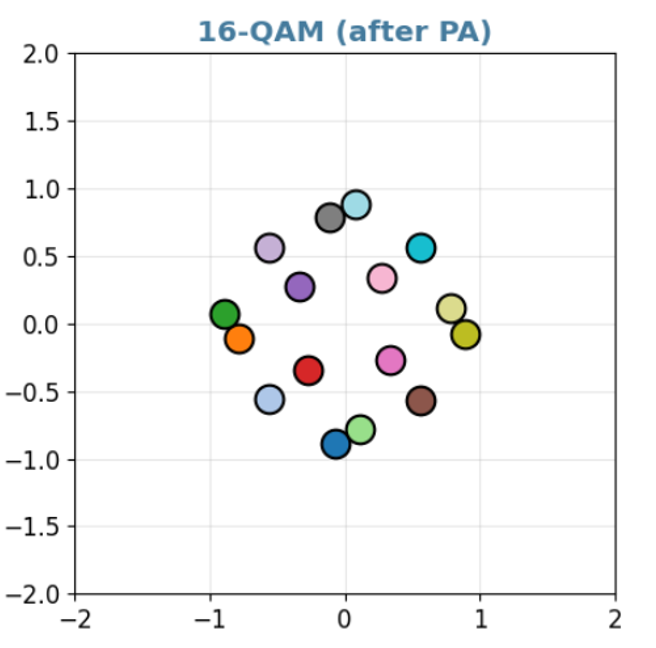
\includegraphics[width=0.48\linewidth]{images/16QAM-constellation-afterPA.png}
    \caption{Standard 16-QAM signal constellation before and after PA distortion.}
    \label{fig:qam_pa}
\end{figure}

\subsubsection{Carrier Frequency Offset (CFO)}
Oscillator mismatch between the transmitter and receiver introduces a frequency offset $\Delta f$, causing progressive phase rotation on the received symbol sequence:
\begin{equation}
y_{cfo}[n] = x[n] \cdot e^{j2\pi \Delta f T_s n}
\end{equation}
where $T_s$ is the symbol period. The cumulative phase rotation increases linearly with index $n$, gradually pushing constellation points out of their decision regions. As shown in Fig.~\ref{fig:cfo_effect}, a normalized CFO of $\Delta f \cdot T_s = 0.02$ causes the constellation to trace a continuous arc over 8 time slots.

\begin{figure}[H]
    \centering
    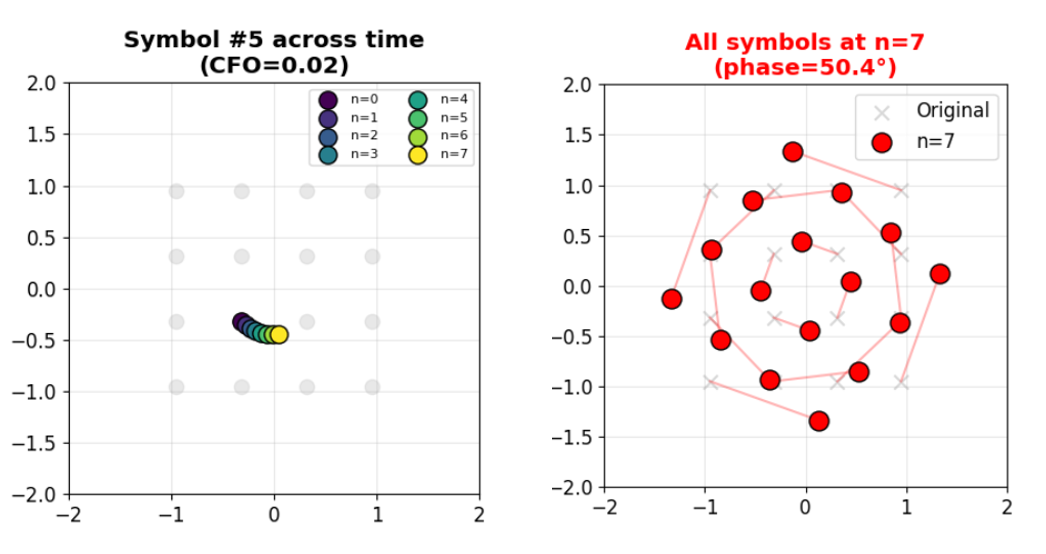
\includegraphics[width=0.98\linewidth]{images/CFO-effect.png}
    \caption{Illustration of CFO causing progressive constellation phase rotation.}
    \label{fig:cfo_effect}
\end{figure}

\subsubsection{Rayleigh Multipath Fading and Inter-Symbol Interference (ISI)}
In multipath environments, the signal reaches the receiver through multiple reflected paths with varying delays and amplitudes. The tapped-delay-line channel model is given by:
\begin{equation}
y[n] = \sum_{l=0}^{L_{ch}-1} h[l] \cdot x[n-l] + w[n]
\end{equation}
where $h[l] \sim \mathcal{CN}(0, \sigma_l^2)$ are Rayleigh-distributed complex channel coefficients, $L_{ch}$ is the number of taps, and $w[n]$ is AWGN.

\subsection{Limitations of Conventional Compensation and the Neural Network Approach}

Conventional systems employ dedicated blocks for each impairment: PLLs for CFO, MMSE/ZF equalizers for ISI, and PAPR reduction before the PA. However, linear equalizers assume $\mathbf{y} = \mathbf{H}\mathbf{x} + \mathbf{w}$, whereas the actual model after PA becomes $\mathbf{y} = \mathbf{H}\phi(\mathbf{x}) + \mathbf{w}$, violating the linearity assumption. Moreover, independent block-wise optimization cannot exploit cross-layer statistical correlations.

Since modulation and demodulation are both nonlinear transformations, deep neural networks (DNNs) offer a natural alternative through their function approximation capability. By modeling the channel as differentiable layers, the entire transceiver can be jointly optimized via backpropagation.

\section{Proposed AutoEncoder Architecture}

\subsection{End-to-End System Model}

\begin{figure}[H]
    \centering
    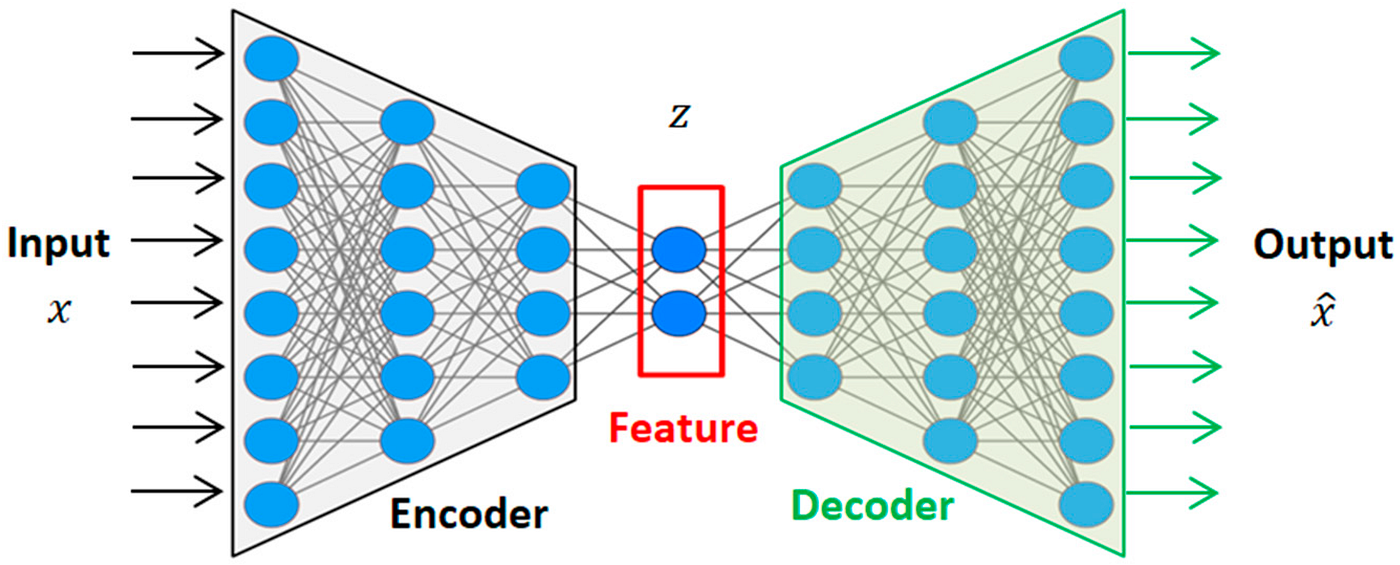
\includegraphics[width=0.78\linewidth]{images/autoencoder.png}
    \caption{Fundamental architecture of the AutoEncoder network.}
    \label{fig:autoencoder}
\end{figure}

The entire digital communication system is modeled as an AutoEncoder network consisting of three components: the Encoder performing dimensionality reduction and mapping input data $\mathbf{x}$ into a latent representation $\mathbf{z}$ for transmission, the Channel Layer which simulates and integrates random physical impairments, and finally the Decoder acting to reconstruct the original transmitted message $\hat{\mathbf{x}}$. The channel is implemented as a differentiable computational layer in TensorFlow, enabling gradient backpropagation from the Decoder through the channel to the Encoder during training.

\begin{figure*}[!t]
    \centering
    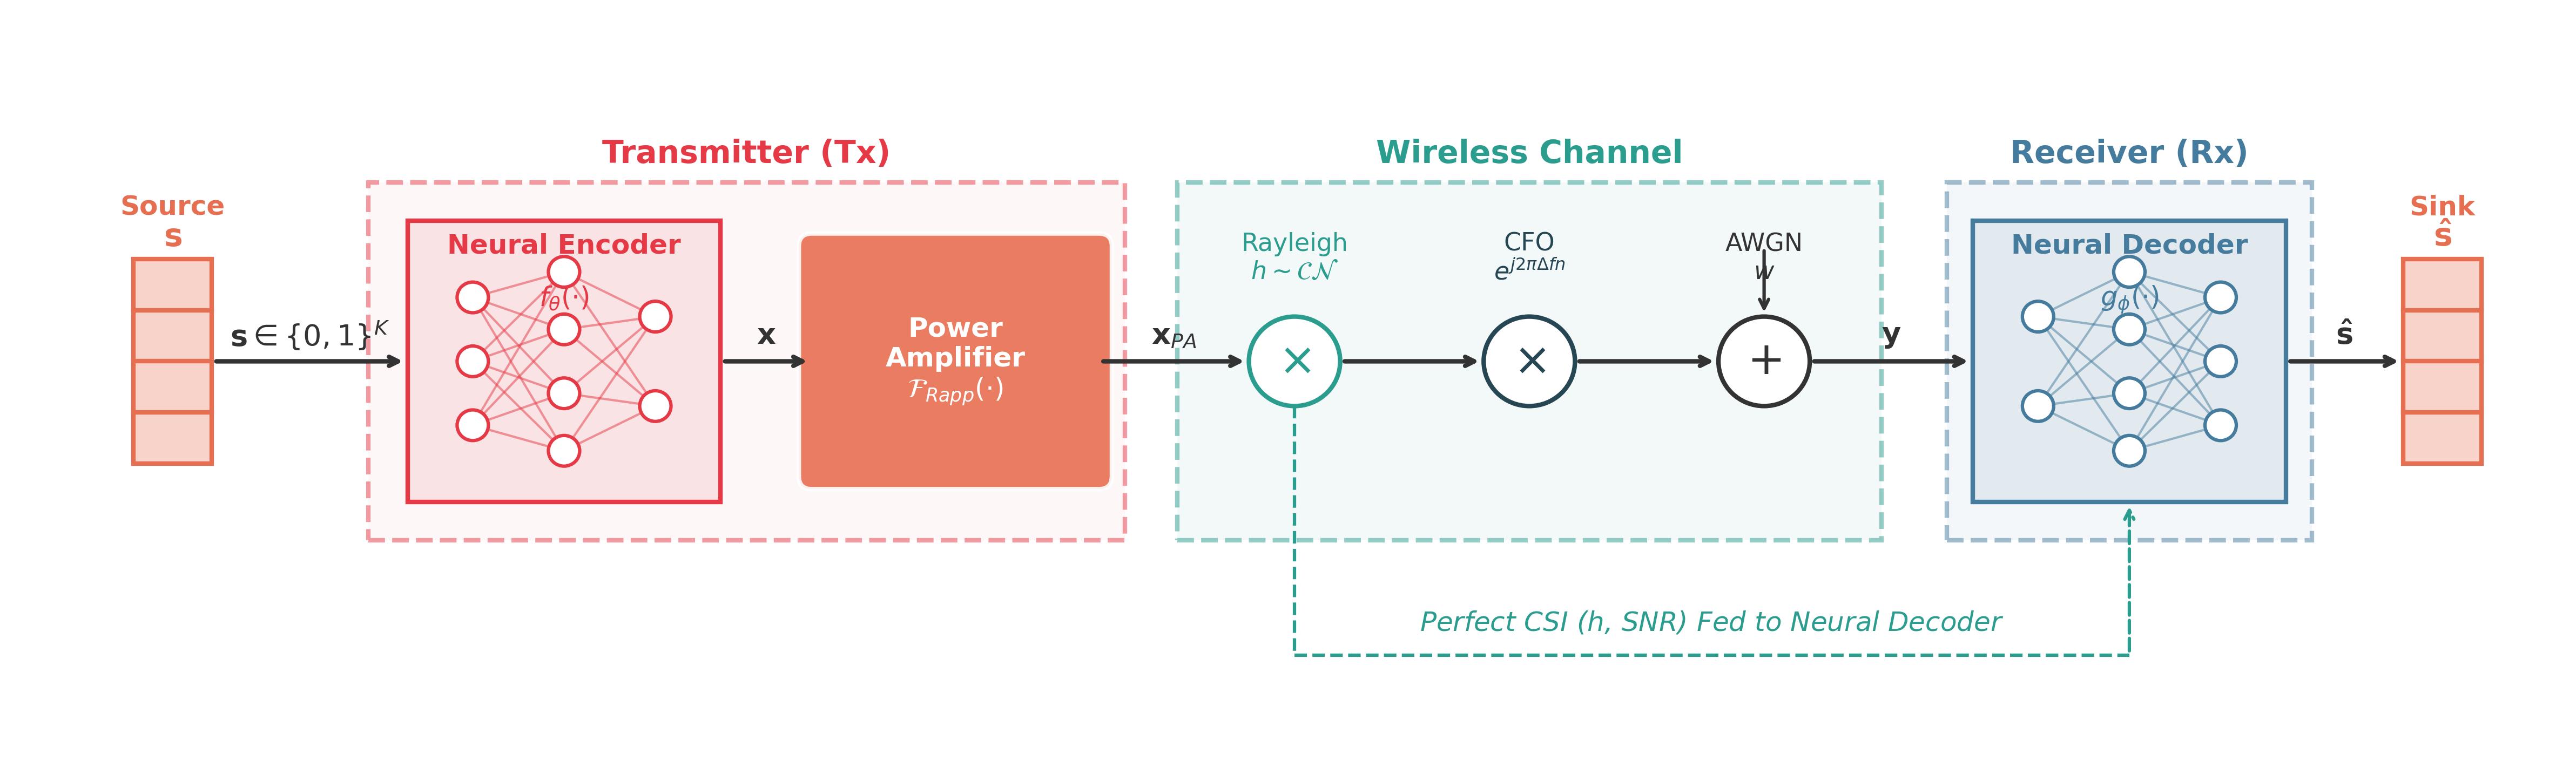
\includegraphics[width=0.95\textwidth]{images/sys_diagram.png}
    \caption{Block diagram of the differentiable End-to-End prototype system.}
    \label{fig:sys_diagram}
\end{figure*}

\subsection{Scenario 1: Single-Symbol AE for PA-Resilient Constellation Shaping}

The first architecture replaces the conventional 16-QAM modulator and demodulator with neural networks. With modulation order $M = 16$, each group of $k = 4$ bits is represented as a one-hot vector $\mathbf{s} \in \{0, 1\}^{M}$ serving as the Encoder input.

The \textbf{Encoder} consists of two FC layers ($64 \to 32$ neurons, ReLU activation), followed by an output layer producing 2 real values representing the I and Q components, using $\tanh$ activation to bound the amplitude. A power normalization layer ensures unit average power:
\begin{equation}
\mathbf{x}_{norm} = \frac{\mathbf{x}_{raw}}{\sqrt{\mathbb{E}[\|\mathbf{x}_{raw}\|^2] + \epsilon}}
\end{equation}
{\color{blue}where $\epsilon > 0$ is a numerical stability constant (typically $\epsilon = 10^{-7}$).}

The \textbf{Channel Layer} sequentially applies: (1) PA nonlinear distortion using the Rapp model; (2) flat Rayleigh fading with $h \sim \mathcal{CN}(0,1)$; (3) AWGN noise; and (4) random phase rotation emulating CFO. The channel output is the raw, unequalized signal $[y_I, y_Q, h_I, h_Q]$---including CSI provided to the Decoder.

The \textbf{Decoder} takes as input the concatenated vector $[y_I, y_Q, h_I, h_Q, SNR]$ (5 dimensions) and passes through FC layers ($256 \to 128$ neurons) combined with Batch Normalization and ReLU activation, terminated by an $M$-class Softmax layer. The Decoder jointly learns equalization and demodulation without requiring a separate ZF/MMSE equalizer block.

\subsection{Scenario 2: Multiple-Symbol Sequence AE for Blind CFO Compensation}

To handle the progressive phase rotation $y_{cfo}[n] = x_{pa}[n] \cdot e^{j2\pi\Delta f T_s n}$ caused by CFO on consecutive symbols, the architecture is extended to a multiple-symbol processing mode. The Encoder simultaneously processes a block of $L$ symbols (e.g., $L = 4$ or $L = 8$).

The \textbf{Encoder} utilizes a Time-Distributed architecture to share weights across symbols within the block: each symbol passes through the same MLP ($256 \to 128 \to 2$ neurons, SELU activation, with Batch Normalization), producing $L$ IQ points with identical statistical properties. The input is a one-hot tensor $\mathbf{S} \in \{0,1\}^{L \times M}$, and the output is $\mathbf{X} \in \mathbb{R}^{L \times 2}$.

The \textbf{Channel Layer} applies Rapp PA distortion per symbol, then generates cumulative CFO phase rotation according to the time index $n \in [0, L-1]$, and finally adds AWGN. The normalized CFO value $\Delta f \cdot T_s$ is randomly sampled during training but is \emph{not} provided to the Decoder---forcing the network to perform blind estimation.

The \textbf{Decoder} receives the entire block of $L$ received symbols by flattening the $(L \times 2)$ tensor into a $2L$-dimensional vector, concatenating normalized SNR, then passing through deep FC layers ($512 \to 512 \to 256 \to 128$ neurons, SELU activation) with Batch Normalization, Dropout, and an SNR re-injection mechanism between layers. The output consists of $L$ independent Softmax branches, each decoding one symbol in the block. By observing the entire phase rotation pattern across $L$ symbols, the Decoder implicitly estimates the linear phase drift trend and performs blind CFO compensation without PLL or pilot signals.

\begin{figure}[H]
    \centering
    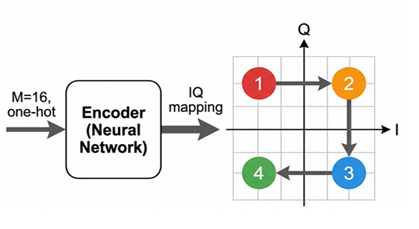
\includegraphics[width=0.7\linewidth]{images/multisymbol Auto Encoder.png}
    \caption{Computational architecture of the shared-sequence TimeDistributed Encoder block.}
    \label{fig:multisymbol_ae}
\end{figure}

\subsection{Scenario 3: Multiple-Symbol AE for Unified Neural FEC}

The third architecture removes the boundary between modulation and channel coding by allowing the Encoder to map $k$ input bits into $N$ IQ symbols, where $N > k / \log_2 M$, creating redundancy analogous to conventional FEC. The code rate is defined as:
\begin{equation}
R = \frac{k}{N \times 2}
\end{equation}
where the factor of 2 accounts for the two real dimensions (I, Q) per symbol.

The \textbf{Encoder} takes the raw bit vector $\mathbf{b} \in \{0, 1\}^k$ directly (without one-hot encoding), passes through two FC layers (64 neurons, ReLU, Batch Normalization), then produces $N \times 2$ real values ($\tanh$ activation), reshaped into a $(N, 2)$ tensor and power-normalized.

The \textbf{Decoder} receives $N$ flattened received symbols, passes through three FC layers ($128 \to 128 \to 64$, ReLU, Batch Normalization), and terminates with $k$ output neurons using Sigmoid activation, directly estimating per-bit probabilities $P(b_i = 1)$. The loss function uses Binary Cross-Entropy combined with a power penalty term.

\subsection{Common Differentiable Channel Layer}

All three architectures share a common differentiable channel model comprising three cascaded components: Rapp PA (Equation~3), CFO (Equation~4), and AWGN.

End-to-End optimization relies on backpropagation, which requires the channel model to be differentiable. A non-differentiable channel block would prevent error gradients from flowing back from the receiver to the transmitter. To address this, the physical channel impairments---PA nonlinearity, CFO, and AWGN---are implemented as a custom differentiable computation layer in TensorFlow, allowing gradient propagation throughout the entire system during training.

\section{Training Methodology}

Training an End-to-End AutoEncoder on complex nonlinear channels poses significant challenges: directly initializing with the full impairment range causes gradient divergence and traps network weights in poor local minima.

\subsection{Curriculum Learning}

The core idea is to utilize curriculum learning{\color{blue}~\cite{bengio2009}} by partitioning the training process into multiple phases of increasing difficulty. This allows the network to establish basic latent representations before introducing severe channel conditions.

\textbf{Scenario 1} (single-symbol AE) employs 3 phases:
\begin{itemize}
    \item \emph{Phase 1 (Constellation shaping):} High SNR ($15$--${\color{blue}35}$~dB), 20 epochs, large learning rate ($3 \times 10^{-3}$).
    \item \emph{Phase 2 (Moderate noise):} SNR expanded to medium ($5$--${\color{blue}35}$~dB), 20 epochs, learning rate ($1 \times 10^{-3}$).
    \item \emph{Phase 3 (Full range):} SNR expanded ($0$--${\color{blue}35}$~dB), 30 epochs, learning rate ($3 \times 10^{-4}$).
\end{itemize}

\textbf{Scenario 2} (multiple-symbol AE) extends to 4 phases with an additional CFO expansion dimension:
\begin{itemize}
    \item \emph{Phase 1:} High SNR ($14$--${\color{blue}35}$~dB), very small CFO ($\pm 0.005$), learning rate $2 \times 10^{-3}$.
    \item \emph{Phase 2:} Medium SNR ($7$--${\color{blue}35}$~dB), increased CFO ($\pm 0.015$), learning rate $5 \times 10^{-4}$.
    \item \emph{Phase 3:} Full SNR range ($0$--${\color{blue}35}$~dB), maximum CFO ($\pm 0.03$), learning rate $2 \times 10^{-4}$.
    \item \emph{Phase 4 (Refinement):} Parameters maintained, very small learning rate ($5 \times 10^{-5}$).
\end{itemize}

\textbf{Scenario 3} (Neural FEC) uses 3 phases similar to Scenario~2 but simplified, as the Encoder maps raw bits rather than one-hot symbols, enabling faster convergence due to the redundant coding space.

\subsection{Custom Loss Function}

\textbf{Scenarios 1 and 3:}
\begin{equation}
\mathcal{L}_{total} = \mathcal{L}_{CE}(\mathbf{s}, \hat{\mathbf{s}}) + \lambda_P \cdot \mathbb{E}\left[\max\left(\|\mathbf{x}\| - \gamma A_{sat},\ 0\right)^2\right]
\end{equation}
{\color{blue}where $\gamma \in (0, 1]$ is the amplitude threshold coefficient relative to the PA saturation level.}

\textbf{Scenario 2} adds a minimum distance penalty component:
\begin{equation}
{\color{blue}\begin{split}
\mathcal{L}_{total} &= \mathcal{L}_{CE} + \lambda_P \cdot \mathbb{E}\!\left[\max\!\left(\|\mathbf{x}\| - \gamma A_{sat},\, 0\right)^{\!2}\right] \\
&\quad + \lambda_D \cdot \max\!\left(d_{target}^2 - d_{\min}^2,\, 0\right)
\end{split}}
\end{equation}

\subsection{Training Stabilization Techniques}

\begin{itemize}
    \item \textbf{Gradient clipping} ($\|\nabla\| \leq 1.0$): Prevents gradient explosion when signals pass through the nonlinear PA layer.
    \item \textbf{Adaptive Learning Rate Decay:} Automatically reduces the learning rate by a factor of 0.5 when validation loss fails to improve for 5--7 epochs.
    \item \textbf{Early Stopping} (Scenarios 2, 3): Halts training if validation loss does not decrease for 10--15 consecutive epochs.
    \item \textbf{Batch Normalization:} Normalizes activation distributions between layers.
    \item \textbf{Dropout} ($p = 0.05$): Applied in the Scenario~2 Decoder to improve generalization.
\end{itemize}

{\color{blue}\subsection{LLR Extraction and System Compatibility}

A key advantage of the proposed AE architecture is its backward compatibility with existing communication systems. The Softmax output layer of the Decoder provides posterior probabilities $P(s_m | \mathbf{y})$ for each symbol $m \in \{0, \ldots, M-1\}$. From these probabilities, per-bit Log-Likelihood Ratio (LLR) values can be directly extracted:
\begin{equation}
L(b_i) = \ln \frac{\sum_{m: b_i(m)=1} P(s_m | \mathbf{y})}{\sum_{m: b_i(m)=0} P(s_m | \mathbf{y})}
\end{equation}
where $b_i(m)$ denotes the $i$-th bit value in the Gray mapping of symbol $m$. These soft LLR values are fully compatible with modern iterative channel decoders (Turbo, LDPC), enabling seamless integration of the AE module into existing transceiver chains without hardware modifications. This is a critical distinction from purely end-to-end AE approaches, which typically require replacing the entire signal processing pipeline.

The synergy between the curriculum learning framework and soft LLR extraction constitutes a practically significant technical contribution: curriculum learning ensures that the AE network converges to an optimal operating point on complex nonlinear channels, while soft LLR outputs enable the AE system to function as an intelligent soft demodulator that can directly replace conventional demodulators in existing transceiver chains --- including systems already deployed with Turbo or LDPC codes --- without requiring any modifications to the downstream channel decoder.}

\subsection{Training Parameters}

Table~\ref{tab:params} summarizes the key parameters for the three scenarios.

\begin{table}[H]
\caption{Training parameters for the three architectural scenarios.}
\label{tab:params}
\centering
\begin{tabular*}{\columnwidth}{@{\extracolsep{\fill}}lccc}
\toprule
\textbf{Parameter} & \textbf{Sc. 1} & \textbf{Sc. 2} & \textbf{Sc. 3} \\
\midrule
Modulation order $M$ & 16 & 16 & --- \\
Input bits $k$ & 4 & 4 & 4 \\
Symbols/block & 1 & 4--8 & 1--6 \\
Code rate $R$ & 1.0 & 1.0 & 1/3--1 \\
Batch size & 4096 & 4096 & 4096 \\
Curriculum phases & 3 & 4 & 3 \\
$A_{sat}$, $p$ & 1.2, 3 & {\color{blue}1.2, 3} & {\color{blue}1.2, 3} \\
Max CFO ($\Delta f \cdot T_s$) & {\color{blue}0.0} & 0.03 & 0.03 \\
Optimizer & Adam & Adam & Adam \\
\bottomrule
\end{tabular*}
\end{table}

\section{Simulation Results and Evaluation}

This section presents the performance evaluation of the proposed AE system compared to conventional 16-QAM through Bit Error Rate (BER) versus Signal-to-Noise Ratio (SNR) analysis. All experiments use Monte Carlo simulations with identical channel conditions to ensure fair comparison. {\color{blue}The channel model employs the Rapp PA ($A_{sat} = 1.2$, $p = 3$, $\alpha_{PM} = 0.08$) combined with flat block Rayleigh fading and normalized CFO $\Delta f \cdot T_s$. The 16-QAM reference receiver uses a Zero-Forcing (ZF) equalizer with a standard grid slicer, with no prior knowledge of PA distortion.}

\subsection{Scenario 1: Single-Symbol AE on Rayleigh + PA Channel}

As illustrated in Fig.~\ref{fig:learned_constellation}, unlike the fixed grid of conventional 16-QAM, the AE learns a flexible constellation geometry.

\begin{figure}[H]
    \centering
    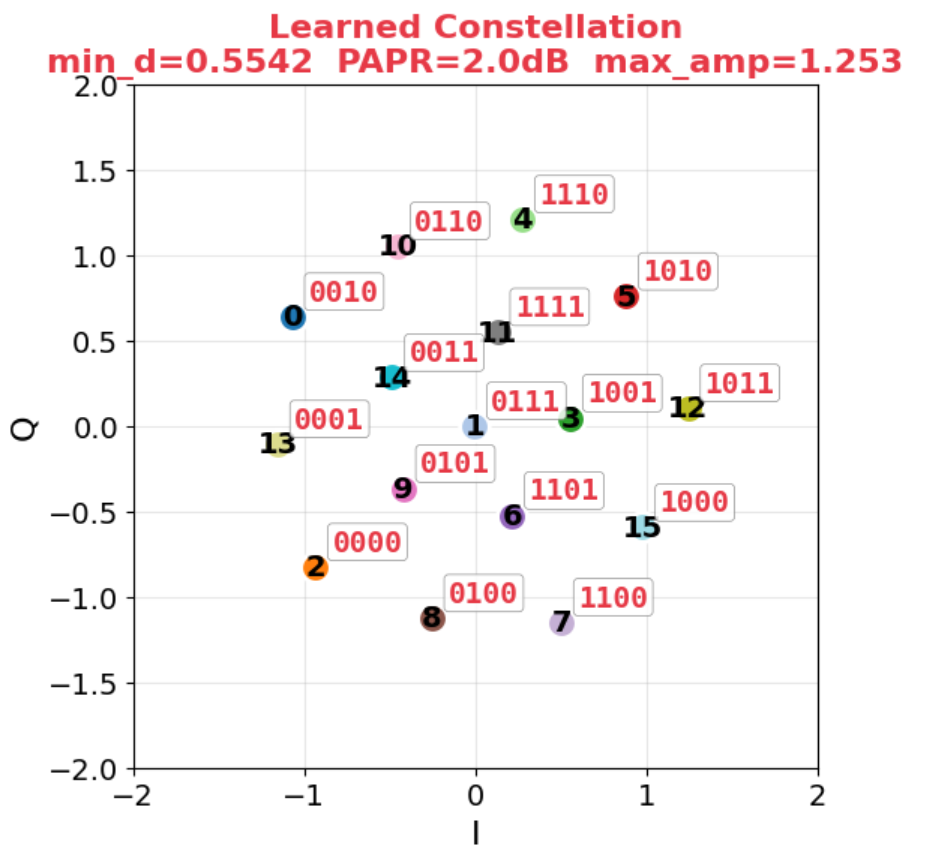
\includegraphics[width=0.85\linewidth]{images/AE-learned-consteallation.png}
    \caption{Self-learned signal constellation block formed by the Encoder.}
    \label{fig:learned_constellation}
\end{figure}

Through end-to-end learning, the Encoder minimizes PA distortion by placing most symbols within the PA's linear region, reducing PAPR from 2.6~dB to approximately 2.3~dB.

\begin{figure}[H]
    \centering
    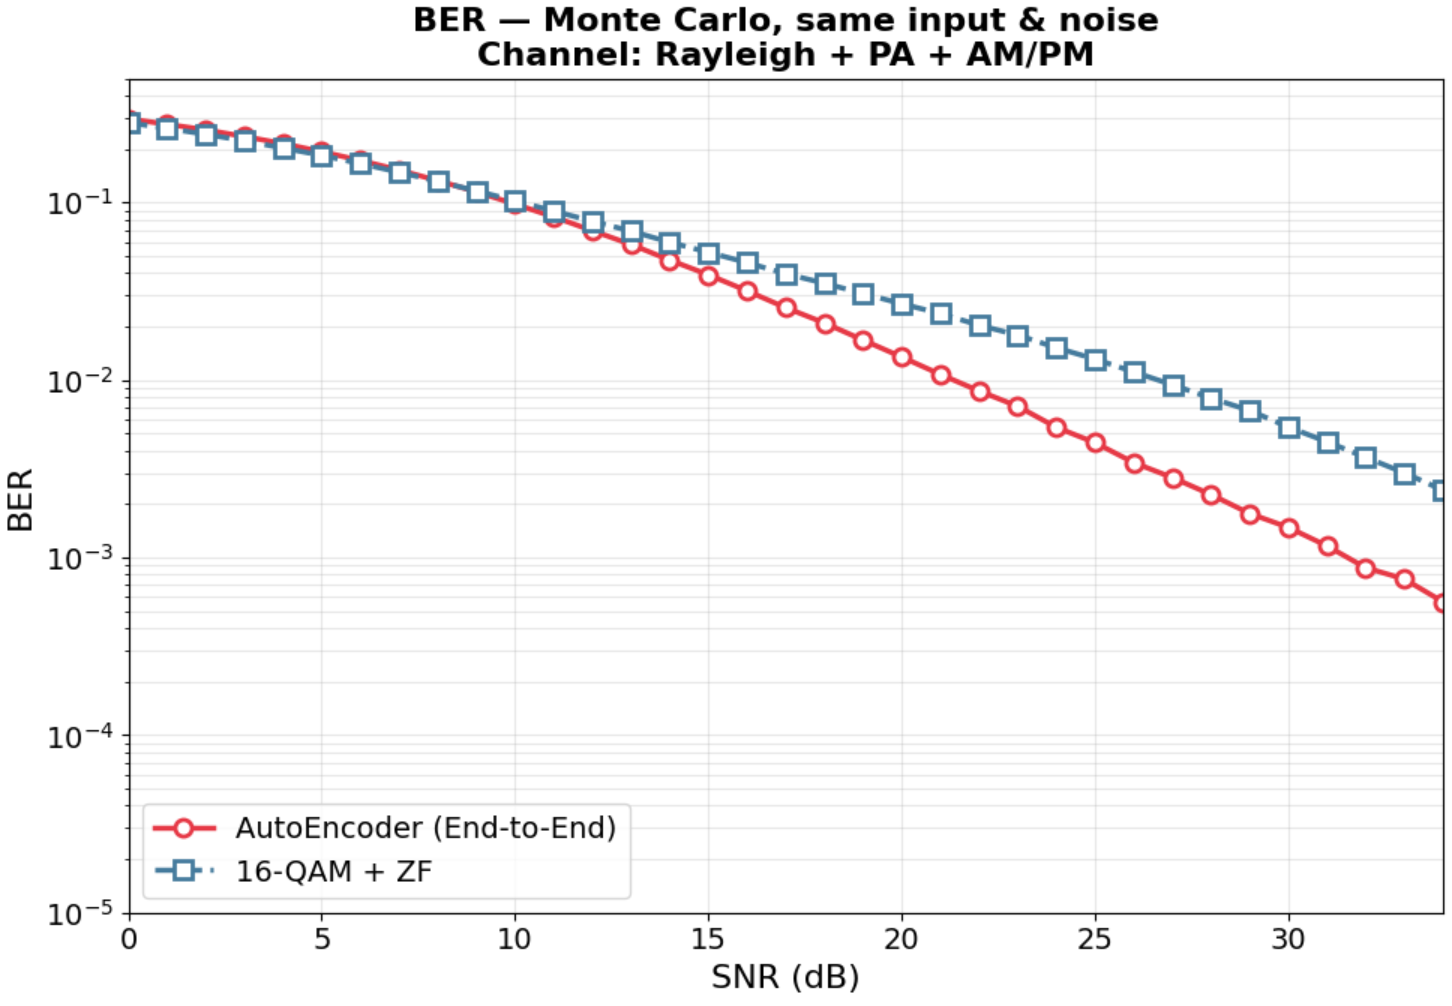
\includegraphics[width=0.95\linewidth]{images/Scenario 1 result-BER AE vs 16QAM .png}
    \caption{BER comparison: AE vs.\ 16-QAM {\color{blue}+ ZF on Rayleigh + PA + AWGN channel}.}
    \label{fig:ber_scenario1}
\end{figure}

{\color{blue}At low SNR ($\leq 12$~dB), both systems exhibit comparable performance. From SNR $\geq 14$~dB onward, the AE demonstrates a clear advantage over 16-QAM + ZF. Specifically, at a target BER~$= 10^{-2}$, the AE provides approximately $3$--$4$~dB SNR gain. Due to Rayleigh fading characteristics (diversity order = 1), both BER curves decrease as $\sim 1/\text{SNR}$ rather than exponentially as in pure AWGN. At SNR = 34~dB, the AE achieves BER $\approx 6 \times 10^{-4}$ while 16-QAM + ZF only reaches $\approx 2.5 \times 10^{-3}$, representing approximately a $4\times$ BER improvement.}

{\color{blue} This performance advantage at high SNR stems from the AE's ability to intuitively internalize the Rapp PA model's non-linear compression curve during the end-to-end training. Unlike the fixed rectangular grid of conventional 16-QAM---which places outer symbols symmetrically, inevitably leading to severe amplitude clipping---the AE dynamically redistributes its constellation points to create a non-uniform geometric structure. It preferentially concentrates symbols closer to the origin and deliberately warps the outer bounds to tolerate the deterministic amplitude compression, effectively shifting the limiting bottleneck from non-linear distortion back to additive noise. At low SNR, where AWGN becomes the dominant impairment rather than PA clipping, the AE's compressed constellation yields comparable performance to 16-QAM since both systems are fundamentally limited by the noise floor.}

\subsection{Scenario 2: Multiple-Symbol AE with Blind CFO Compensation}

This scenario evaluates the blind CFO compensation capability of the multi-symbol AE ($L = 4$).

\begin{figure}[H]
    \centering
    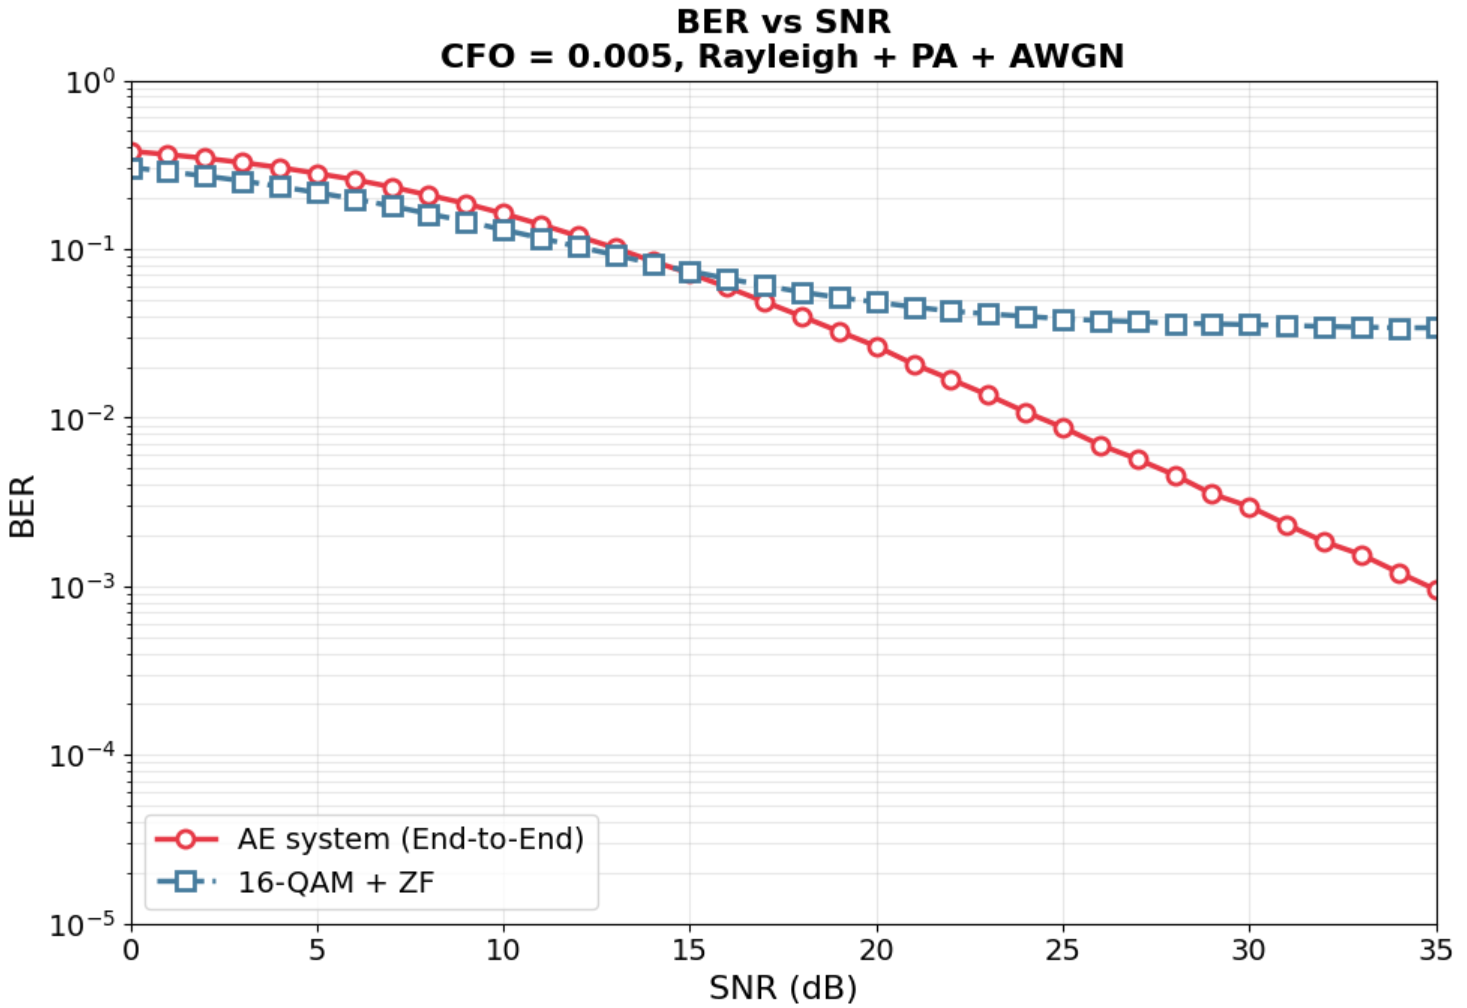
\includegraphics[width=0.95\linewidth]{images/Scenario 2 result-BER AE vs 16QAM CFO 0.005 .png}
    \caption{{\color{blue}BER on Rayleigh + PA + CFO + AWGN channel at $\Delta f \cdot T_s = 0.005$.}}
    \label{fig:ber_cfo005}
\end{figure}

\begin{figure}[H]
    \centering
    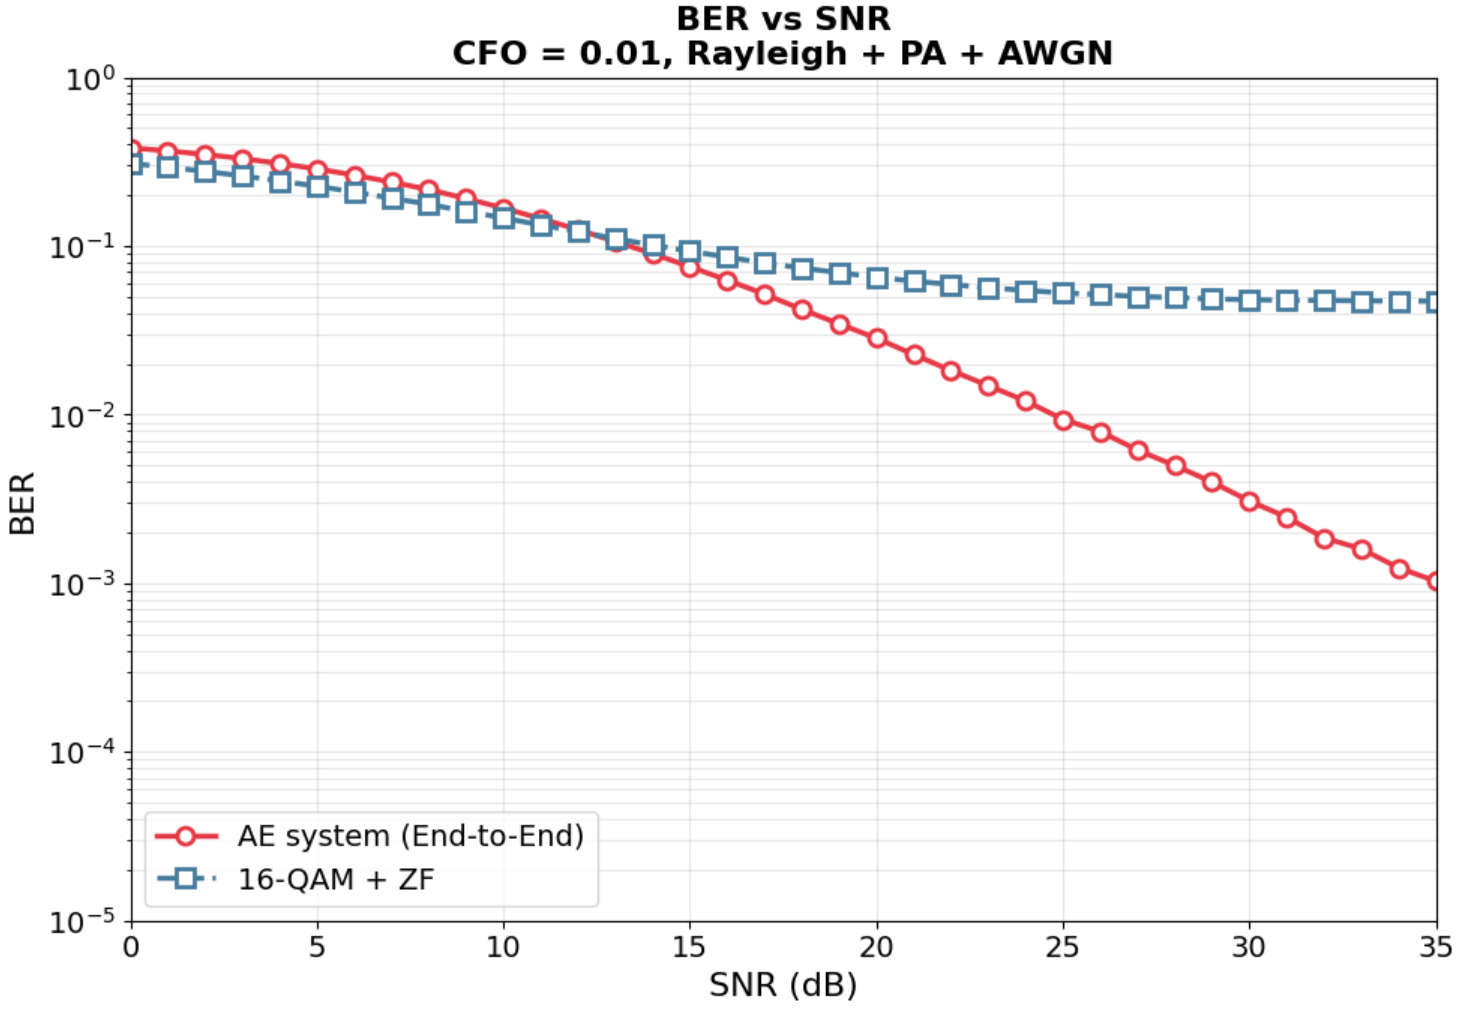
\includegraphics[width=0.95\linewidth]{images/Scenario 2 result-BER AE vs 16QAM CFO 0.01 .png}
    \caption{{\color{blue}BER on Rayleigh + PA + CFO + AWGN channel at $\Delta f \cdot T_s = 0.01$.}}
    \label{fig:ber_cfo01}
\end{figure}

{\color{blue}As shown in Fig.~\ref{fig:ber_cfo005} and Fig.~\ref{fig:ber_cfo01}, in the presence of CFO, the 16-QAM + ZF system (without CFO compensation) rapidly reaches an error floor due to progressive phase rotation destroying the grid-based decoding: at CFO = 0.005, QAM BER saturates at $\approx 3 \times 10^{-2}$ for SNR $\geq 18$~dB; at CFO = 0.01, the floor rises to $\approx 5 \times 10^{-2}$. In contrast, the AE continues to decrease BER to $\approx 10^{-3}$ at SNR = 35~dB through its blind CFO estimation from the symbol sequence. At BER~$= 10^{-2}$, the AE achieves approximately $5$--$8$~dB gain over 16-QAM + ZF at both CFO levels.}

Table~\ref{tab:cfo_comparison} summarizes BER at representative SNR and CFO values.

\begin{table}[H]
\caption{BER comparison at SNR = 20 dB across CFO values.}
\label{tab:cfo_comparison}
\centering
\begin{tabular*}{\columnwidth}{@{\extracolsep{\fill}}lcc}
\toprule
\textbf{CFO} & \textbf{AE (blind)} & {\color{blue}\textbf{16-QAM + ZF}} \\
\midrule
{\color{blue}0.0}    & {\color{blue}$\approx 1.0 \times 10^{-2}$} & {\color{blue}$\approx 1.5 \times 10^{-2}$} \\
{\color{blue}0.005}  & {\color{blue}$\approx 1.2 \times 10^{-2}$} & {\color{blue}$\approx 3.0 \times 10^{-2}$} \\
{\color{blue}0.01}   & {\color{blue}$\approx 1.5 \times 10^{-2}$} & {\color{blue}$\approx 5.0 \times 10^{-2}$} \\
\bottomrule
\end{tabular*}
\end{table}

{\color{blue}The AE demonstrates a clear advantage across all evaluated CFO levels: at CFO = 0, the AE achieves lower BER than 16-QAM + ZF due to its PA distortion compensation capability; as CFO increases, the performance gap widens significantly since 16-QAM + ZF lacks any CFO compensation mechanism and quickly reaches an error floor, while the AE implicitly estimates and compensates CFO from the phase rotation pattern across the $L$-symbol block.}

{\color{blue} This blind compensation capability intrinsically stems from the Time-Distributed encoder, which generates a correlated sequence of symbols that implicitly encodes relative phase information across the entire block. When the progressive CFO uniformly rotates this block during transmission, the deep neural decoder functions as an advanced non-linear sequence pattern recognizer. Rather than explicitly computing phase derivatives like a conventional PLL, the decoder simultaneously observes the overarching arched trajectory of the 4 received symbols. The dense fully connected layers effectively map this rotational path back to the original discrete sequence. This block-level, holistic decision-making provides strong robustness against transient noise spikes that would otherwise induce catastrophic phase-slips in a traditional PLL tracking loop.}

\subsection{Scenario 3: AE with Neural Forward Error Correction}

{\color{blue}By allowing the Encoder to map $k=4$ input bits into $N$ IQ symbols (with $N > 1$), the proposed system can implicitly embed forward error correction.} Fig.~\ref{fig:ber_scenario3} compares BER across different code rate configurations on the PA+CFO$_{0.02}$+AWGN channel.

\begin{figure}[H]
    \centering
    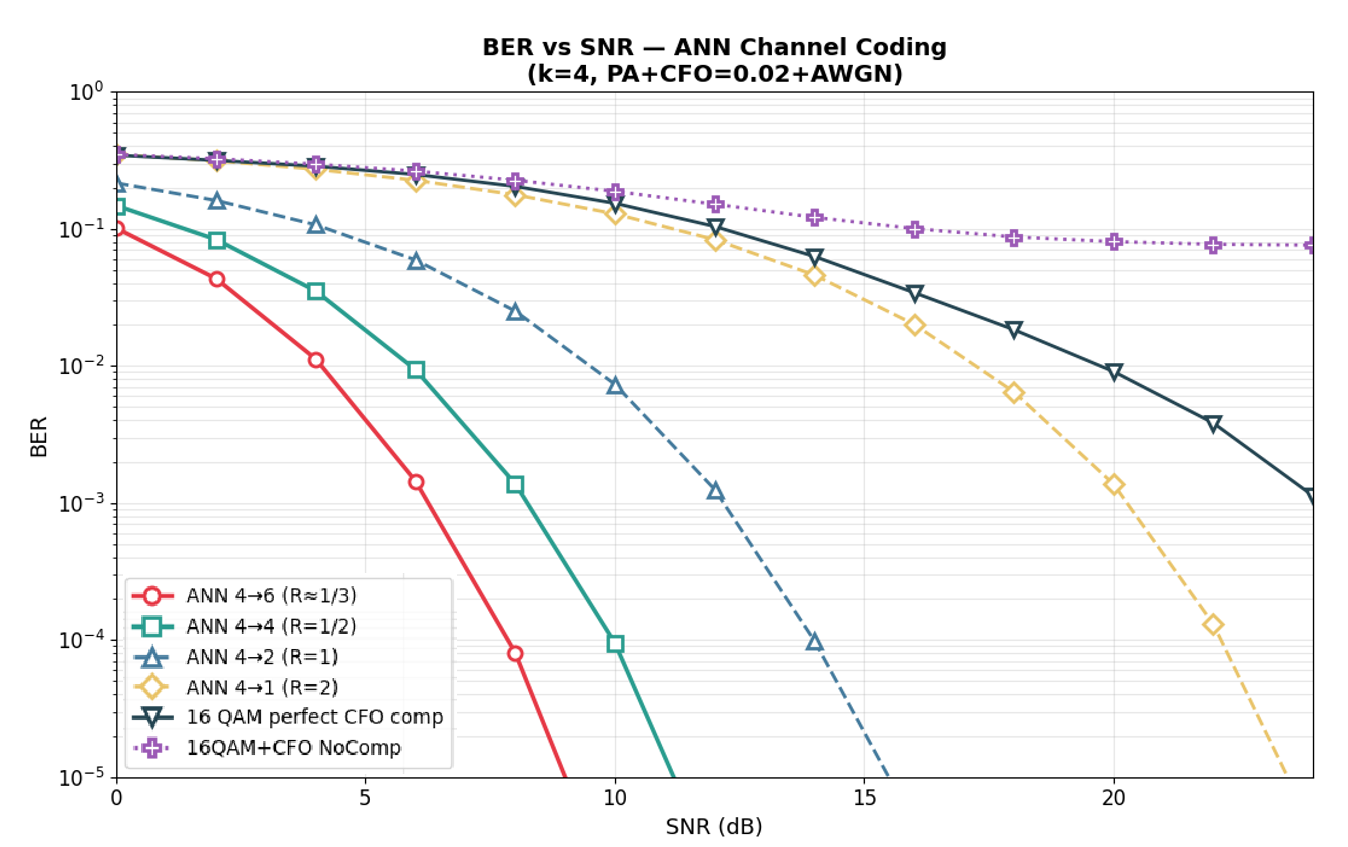
\includegraphics[width=0.98\linewidth]{images/Scenario 3 AE with channel coding feature .png}
    \caption{AE system performance with FEC coding functionality.}
    \label{fig:ber_scenario3}
\end{figure}

The configuration AE $4 \to 6$ ($R \approx 1/3$) demonstrates strong noise resilience, reaching BER~$< 10^{-4}$ at SNR~$\approx$~8~dB, confirming successful channel coding by the neural network.

{\color{blue} This error correction performance is explained by the network's ability to autonomously form a unified coding space that bridges the Hamming and Euclidean domains. While traditional transceivers strictly partition the Hamming space (bit redundancy for FEC) from the Euclidean space (IQ modulation), the Neural FEC generates continuous analog waveforms that inherently maximize the Euclidean distance over multiple combined time steps. Instead of making intermediate bit-level decisions at each stage, the network distributes the information content of the 4 input bits across all 6 transmitted IQ symbols. This information diversity mechanism ensures that even when one or two symbols are severely degraded by deep fading or CFO-induced phase rotation, the remaining symbols retain sufficient redundant information for the decoder to accurately recover the original message.}

\subsection{Summary Discussion}

Table~\ref{tab:summary} consolidates the strengths and limitations of the AE architecture across all three scenarios.

\begin{table}[H]
\caption{Summary of AE system advantages and limitations vs.\ conventional 16-QAM.}
\label{tab:summary}
\centering
\begin{tabular*}{\columnwidth}{@{\extracolsep{\fill}}p{1.4cm}p{3.0cm}p{2.6cm}}
\toprule
\textbf{Criterion} & \textbf{AE Advantage} & \textbf{AE Limitation} \\
\midrule
PA Resil. & Self-learned PA-resilient constellation, PAPR $-$0.3~dB & Worse than QAM at low SNR \\
CFO Comp. & {\color{blue}Blind comp. without PLL/pilot, 5--8~dB gain over QAM+ZF when CFO $> 0$} & {\color{blue}BER decreases slowly due to Rayleigh} \\
FEC & Neural FEC performs channel coding well & Reduced spectral efficiency \\
Design & No per-block engineering needed & Complex curriculum training \\
\bottomrule
\end{tabular*}
\end{table}

{\color{blue}Ultimately, the proposed AE architecture demonstrates its primary advantage on complex composite channels (PA + CFO + Rayleigh), where independent block-wise processing of conventional systems is sub-optimal.}

\section{Conclusion}

{\color{blue}This paper has presented and evaluated an End-to-End digital communication system based on deep AutoEncoder networks, demonstrating its potential to improve performance over conventional communication systems when deployed over complex, composite non-ideal wireless channels. The research demonstrates three major contributions. First, the AE autonomously learns a PA-resilient non-uniform constellation geometry that optimally mitigates nonlinear amplifier clipping, yielding a $3$--$4$~dB SNR gain over conventional 16-QAM with ZF equalization on Rayleigh + PA channels. Second, by exploiting multi-symbol sequence learning, the decoder intrinsically performs robust blind CFO compensation without the overhead of pilot signals or PLLs, achieving a $5$--$8$~dB gain over 16-QAM + ZF (which lacks CFO compensation). Finally, the proposed architecture successfully unifies digital modulation and forward error correction into a single Neural FEC model, proving that deep neural networks can implicitly internalize and reproduce sophisticated channel coding redundancies.} {\color{blue}In addition, this work contributes a smart training framework based on multi-phase curriculum learning combined with physics-constrained custom loss functions (power penalty and minimum distance regularization), enabling stable AE convergence on complex nonlinear channels --- a challenge that conventional direct training approaches cannot overcome. Notably, the Softmax output design enables soft LLR extraction, allowing the AE module to function as an intelligent soft demodulator that is fully compatible with modern iterative channel decoders (Turbo, LDPC) without requiring any modifications to existing system architectures.} {\color{blue}These results suggest that deep learning-based joint transceivers hold significant potential as an effective alternative to conventional block-wise signal processing approaches, particularly over strongly nonlinear channels (PA distortion, CFO, and Rayleigh fading). Future work will expand this framework to incorporate Orthogonal Frequency-Division Multiplexing (OFDM) for frequency-selective multipath channels and investigate Software-Defined Radio (SDR) based experimental deployments, leveraging emerging GPU-accelerated platforms such as the Sionna Research Kit~\cite{cammerer2025} for real-world AI-RAN prototyping.}

\section*{Acknowledgments}
The authors thank the institution for providing research facilities and computational resources.

\begingroup
\small
\begin{thebibliography}{10}
\setlength{\itemsep}{0pt}
\setlength{\parsep}{0pt}
\bibitem{hornik1991}
K.~Hornik, ``Approximation capabilities of multilayer feedforward networks,'' \emph{Neural Networks}, vol.~4, no.~2, pp.~251--257, 1991.
\bibitem{proakis2008}
J.~G.~Proakis and M.~Salehi, \emph{Digital Communications}, 5th~ed. New York: McGraw-Hill, 2008.
\bibitem{oshea2017}
T.~O'Shea and J.~Hoydis, ``An introduction to deep learning for the physical layer,'' \emph{IEEE Trans. Cogn. Commun. Netw.}, vol.~3, no.~4, pp.~563--575, Dec. 2017.

\bibitem{stark2019}
M.~Stark, F.~A.~Aoudia, and J.~Hoydis, ``Joint learning of geometric and probabilistic constellation shaping,'' in \emph{Proc. IEEE GC Wkshps}, 2019, pp.~1--6.
\bibitem{bengio2009}
Y.~Bengio, J.~Louradour, R.~Collobert, and J.~Weston, ``Curriculum learning,'' in \emph{Proc. ICML}, 2009, pp.~41--48.
\bibitem{cammerer2020}
S.~Cammerer, F.~A.~Aoudia, S.~D\"{o}rner, M.~Stark, J.~Hoydis, and S.~ten Brink, ``Trainable communication systems: Concepts and prototype,'' \emph{IEEE Trans. Commun.}, vol.~68, no.~9, pp.~5489--5503, Sep. 2020.
\bibitem{aoudia2022}
F.~A.~Aoudia and J.~Hoydis, ``End-to-end learning for OFDM: From neural receivers to pilotless communication,'' \emph{IEEE Trans. Wireless Commun.}, vol.~21, no.~2, pp.~1049--1063, Feb. 2022.
\bibitem{hoydis2024}
J.~Hoydis, F.~A.~Aoudia, S.~Cammerer, F.~Euchner, M.~Nimier-David, S.~ten Brink, and A.~Keller, ``Learning radio environments by differentiable ray tracing,'' \emph{IEEE Trans. Mach. Learn. Commun. Netw.}, vol.~2, pp.~638--654, 2024.
\bibitem{wiesmayr2025}
R.~Wiesmayr, S.~Cammerer, F.~A.~Aoudia, J.~Hoydis, J.~Zakrzewski, and A.~Keller, ``Design of a standard-compliant real-time neural receiver for 5G NR,'' in \emph{Proc. IEEE ICMLCN}, May 2025.
\bibitem{cammerer2025}
S.~Cammerer, G.~Marcus, T.~Zirr, F.~A.~Aoudia, L.~Maggi, J.~Hoydis, and A.~Keller, ``Sionna Research Kit: A GPU-accelerated research platform for AI-RAN,'' in \emph{Proc. IEEE ICMLCN}, May 2025.
\end{thebibliography}
\endgroup
\vspace{-0.5\baselineskip}
\newcommand{\compactbio}[3]{%
\par\noindent
\begin{minipage}[t]{1.0in}
\vspace{0pt}\includegraphics[width=1in,height=1.25in,clip,keepaspectratio]{#1}
\end{minipage}\hspace{0.14in}%
\begin{minipage}[t]{\dimexpr\columnwidth-1.14in\relax}
\vspace{0pt}\footnotesize\textbf{#2} #3
\end{minipage}\par\vspace{0.25\baselineskip}}
\compactbio{images/authors/Lai_Tien_De_color_photo.jpg}{Lai Tien De}{received the Engineer degree from Le Quy Don Technical University, Hanoi, Vietnam, in 2020. He is currently a Lecturer with the Faculty of Radio-Electronics Engineering, Le Quy Don Technical University. His research interests include information theory, signal processing, wireless communications, and artificial intelligence.}
\compactbio{images/authors/Pham_Xuan_Nghia_color_photo.png}{Pham Xuan Nghia}{received the B.S. and M.S. degrees in information engineering from Le Quy Don Technical University, Hanoi, Vietnam, and the Ph.D. degree in electronics engineering from a university in the Russian Federation. He is currently a Lecturer with the Faculty of Radio-Electronics Engineering, Le Quy Don Technical University. His research interests include information theory, signal processing, and wireless communications.}
\compactbio{images/authors/Tran_Duc_Trung_color_photo.png}{Tran Trung Duc}{received the Engineer and M.S. degrees in information engineering from Le Quy Don Technical University, Hanoi, Vietnam. He is currently working at the Center for Standards, Metrology and Quality. His research interests include information theory, information security, and computer networks.}

\end{document}
